





\documentclass[conference]{IEEEtran}
%
\ifCLASSINFOpdf
  
  % \DeclareGraphicsExtensions{.pdf,.jpeg,.png}
\else
  % or other class option (dvipsone, dvipdf, if not using dvips). graphicx
  % will default to the driver specified in the system graphics.cfg if no
  % driver is specified.
  % \usepackage[dvips]{graphicx}
  % declare the path(s) where your graphic files are
  % \graphicspath{{../eps/}}
  % and their extensions so you won't have to specify these with
  % every instance of \includegraphics
  % \DeclareGraphicsExtensions{.eps}
\fi






% correct bad hyphenation here
\hyphenation{op-tical net-works semi-conduc-tor}
\usepackage{listings}

\usepackage{xcolor}
\usepackage{graphicx}
\graphicspath{ {./images/} }



\definecolor{codegreen}{rgb}{0,0.6,0}
\definecolor{codegray}{rgb}{0.5,0.5,0.5}
\definecolor{codepurple}{rgb}{0.58,0,0.82}
\definecolor{backcolour}{rgb}{0.95,0.95,0.92}

\lstdefinestyle{mystyle}{
    backgroundcolor=\color{backcolour},   
    commentstyle=\color{codegreen},
    keywordstyle=\color{magenta},
    numberstyle=\tiny\color{codegray},
    stringstyle=\color{codepurple},
    basicstyle=\ttfamily\footnotesize,
    breakatwhitespace=false,         
    breaklines=true,                 
    captionpos=b,                    
    keepspaces=true,                 
    numbers=left,                    
    numbersep=5pt,                  
    showspaces=false,                
    showstringspaces=false,
    showtabs=false,                  
    tabsize=2
}

\usepackage{color}

\definecolor{mygreen}{rgb}{0,0.6,0}
\definecolor{mygray}{rgb}{0.5,0.5,0.5}
\definecolor{mymauve}{rgb}{0.58,0,0.82}

\lstset{ 
  backgroundcolor=\color{white},   % choose the background color; you must add \usepackage{color} or \usepackage{xcolor}; should come as last argument
  basicstyle=\footnotesize,        % the size of the fonts that are used for the code
  breakatwhitespace=false,         % sets if automatic breaks should only happen at whitespace
  breaklines=true,                 % sets automatic line breaking
  captionpos=b,                    % sets the caption-position to bottom
  commentstyle=\color{mygreen},    % comment style
  deletekeywords={...},            % if you want to delete keywords from the given language
  escapeinside={\%*}{*)},          % if you want to add LaTeX within your code
  extendedchars=true,              % lets you use non-ASCII characters; for 8-bits encodings only, does not work with UTF-8
  frame=single,	                   % adds a frame around the code
  keepspaces=true,                 % keeps spaces in text, useful for keeping indentation of code (possibly needs columns=flexible)
  keywordstyle=\color{blue},       % keyword style
  language=Octave,                 % the language of the code
  morekeywords={*,...},            % if you want to add more keywords to the set
  numbersep=5pt,                   % how far the line-numbers are from the code
  numberstyle=\tiny\color{mygray}, % the style that is used for the line-numbers
  rulecolor=\color{black},         % if not set, the frame-color may be changed on line-breaks within not-black text (e.g. comments (green here))
  showspaces=false,                % show spaces everywhere adding particular underscores; it overrides 'showstringspaces'
  showstringspaces=false,          % underline spaces within strings only
  showtabs=false,                  % show tabs within strings adding particular underscores
  stepnumber=2,                    % the step between two line-numbers. If it's 1, each line will be numbered
  stringstyle=\color{mymauve},     % string literal style
  tabsize=2,	                   % sets default tabsize to 2 spaces
  title=\lstname                   % show the filename of files included with \lstinputlisting; also try caption instead of title
}

\lstdefinestyle{customc}{
  belowcaptionskip=1\baselineskip,
  breaklines=true,
  frame=L,
  xleftmargin=\parindent,
  language=C,
  showstringspaces=false,
  basicstyle=\footnotesize\ttfamily,
  keywordstyle=\bfseries\color{green!40!black},
  commentstyle=\itshape\color{purple!40!black},
  identifierstyle=\color{blue},
  stringstyle=\color{orange},
}

\lstdefinestyle{customasm}{
  belowcaptionskip=1\baselineskip,
  frame=L,
  xleftmargin=\parindent,
  language=[x86masm]Assembler,
  basicstyle=\footnotesize\ttfamily,
  commentstyle=\itshape\color{purple!40!black},
}

\lstset{escapechar=@,style=customc}



\providecommand{\keywords}[1]
{
  \small	
  \textbf{\textit{Keywords---}} #1
}



\begin{document}
%
% paper title

\title{Implement KNN Classifier for Sequence Prediction}


% author names and affiliations
% use a multiple column layout for up to three different
% affiliations
\author{\IEEEauthorblockN{Dr.Muhammad Haris}
\IEEEauthorblockA{Information Technology (M.Eng.)\\Computer Science and Engineering\\
Frankfurt University of Applied Sciences\\
Frankfurt am Main, Germany\\
Email: here}
\and
\IEEEauthorblockN{Zaka Ahmed}
\IEEEauthorblockA{Information Technology (M.Eng.)\\Computer Science and Engineering\\
Frankfurt University of Applied Sciences\\
Frankfurt am Main, Germany\\
zaka.ahmed@stud.fra-uas.de}}




% make the title area
\maketitle

% As a general rule, do not put math, special symbols or citations
% in the abstract
\begin{abstract}
Machine Learning (ML) has become ubiquitous in various industries and evolving in our daily life. The sectors in which machine learning is involved include education, Telecommunication, retail, research and development, finance, healthcare and transportation. As, the development is going on various algorithms are used for prediction of text, images, videos and pictures. 

There are various classifier aviliable including support vector machines, decision trees, naive Bayes, and K-Nearest Neighbours for data analysis. In this paper, our main focus is on KNN Implementation for sequence prediction with Hierarchical Temporal Memory (HTM). Supervised learning enables the prediction of output variables based on the input. Hierarchical Temporal Memory offers capabilities to learn complex temporal patterns, making it well-suited for processing sequential data. The Neocortex API helps in the integration of KNN model with HTM, which enables efficient classification of the sequences. 

We are using three inputs odd numbers, even numbers or neither odd or even. These sequences are encoded and mapped on the cells which gives us SDR values. These SDR active cells are our data inputs. Which are further disguinsh by 0.3 in testing data and 0.7 in training data. Meaning splitting the dataset into two parts. Where 80\% belongs to training data and other 20\% to test data. Remember Training and testing data is labeled but while testing last index is not considered. In the further steps, using the Input SDR we will find the distance matrix between the training and test data. And then using K and voting method. We decide whether the unlabed data is belongs to that specific class. In KNN classification, the object is classified based on the votes of its nearest neighbors. If k=1, then the object will be in the class of that single nearest neighbor.The simple function of the kNN model is to predict the target class
label. This is further explained in the paper. 

The results achieved has shown a 80\% accuracy rate in classifying the input sequences. In this paper we covers the introduction and important parameters of K-Nearest, Distance Matrics, KNN impelementation, and the challenges regarding KNN.  






\end{abstract}\hspace{10pt}

\keywords{Machine Learning, Hierarchical Temporal Memory, K-Nearest Neighbors, Sequence Classification, Integration, Neocortex API, Accuracy Enhancement}





\IEEEpeerreviewmaketitle



\section{Introduction}

\subsection{Background}
KNN was first developed by Joseph Hodges and Evelyn Fix in the year 1951[1], in statistics the concept of k-nearest neighbors algorithm(k-NN) is involved in the non-parametric supervised learning method. Further developments in KNN are proceeded by Thomas Cover.[2]  KNN is commonly used for regression and classification. Both in regression and classification the input consists of k-closest training examples in the data set. Remember the output depends on whether the use case is either regression or classification of K-NN. 

\subsection{Regression}
The main difference between classification and regression is that in regression, the output is the property value for the object. The value is the total average of the neighbor's nearest values. If k=1, the output is assigned from that particular single nearest neighbor. 

\subsection{Classification}
The main variation in the output of classifier and regression is that in classification, the output is the class membership. In classification, the object is classified based on the votes of its nearest neighbors. If k = 1, then the object will be in the class of that single nearest neighbor. The simple function of the kNN model is to predict the target class label. In other words, the class label is often described as a majority voting. The most common terms are technically considered "plurality voting" and "majority vote" The term "majority voting" means the majority needs to be greater the 50\%  
for making decisions. The classification problems with only two classes, like binary predictions, there is always a majority. A majority vote is also automatically a plurality vote. We don't require multi-class settings to make predictions via kNN in multi-class settings. 




\section{Methods}

This section includes multiple subsections including description of KNN in detail, second section try to focus on Theoretical background of including how the values determined accuracy and complexity  of the classifier. In the last section of this section is regarding Hierarchical temporal Memory(HTM). 



\subsection{Literature Review}
The K-Nearest Neighbors (KNN) algorithm is a widely-used non-parametric classification method in machine learning. KNN depend on instance based learning where prediction is made based on the similarity of new data points to existing labeled data points. In finance, KNN is used for credit scoring, stock analysis and fraud detection. In healthcare sector, KNN is used for patient health monitoring and drug suggestions. If, I will talk about marketing professionally KNN is used as product suggestion, market trend analysis and customer ads suggestions. In most cases KNN is used for determining the specific patterns and tasks like face recognition or image classification. 

Researchers have proposed various enhancements to the traditional KNN algorithm which can improve the scalability and performance. The weight adjustment algorithm is proposed by Han EH., proposed assigning weights to the nearest neighbors based on their distance from the respective point.[11][8]. The assigned weights desgunish, how much the weights influence the classification method. In this way, high weights will be assigned to the one who are closer neigbors, so it give more priority to the similar instances while performing classification.  This technique is usefull where the dataset has many feature, some of which can be considered as unneccessary but it has high cost in context of computational cost.

Zhang et al. has proposed to adjust the value of K based on the local density of data points [3]. This adaptive KNN algorithm dynamically selects the optimal value of K for each query point, leading to more robust predictions. And shows that the adaptive algorithm outperforms many other traditional KNN algorithms. The other approach can be locally adoptive KNN algorithm. It choices the optimal value of K for classifying an input by analyzing the outcomes of cross-validation computations within the local neighborhood of the unlabeled data point.[12]  The approach defined by Song Yang, is to introduce two input parameters. As we know determining the correct value of K depends on the characteristics of the dataset, the selection of correct parmeter for various applications is a challenge. Song Yang suggest to introduce a novel metric that assesses the informativeness of objects to be classified, with informativeness quantifying the significance of data points. 
Two parameter will be K and I as a input. The class is determined based on the majority class of the most informative training examples.[10]

Whereas on the some has proposed to integrated KNN with dimensionality reduction methods such as principal component analysis (PCA) to improve computational efficiency [5]. This a combination is a example of hybrid approach. Whereas other have combined KNN with ensemble methods such as random forests to enhance predictive accuracy [6]. These hybrid approaches enhance the performance as compared to standalone KNN. 








\subsection{K-Nearest Neighbors Parameters and Materics}
The K-nearest was first used by US Air force to execute characteristics analysis. There are differnet paramenters in KNN classsifier which plays a important role in algorithm designs including distance matrics, K-Value selection, and voting. 




\subsubsection{Computing Distance Matrics}
If we try to recap, the main objective of the k-nearest neighbor algorithm is the identification of the nearest neighbors of a given input point. So, What we can do is assign a class label to that specific point. The first thing is determining the distance matrics. In order to find which class(data point) is nearest to the input data, to do so we will calculate the distance between the data points and query point. We get assistance to decide in which regions the input point belongs. The distance metrics can be either Manhattan distance or any other approach. The first thing is to indentify the k-nearest neighbors and then amount of its k-neatest neighbors.The most famous techniques are discussed below:  


\paragraph{\textbf{Euclidean distance (p=2)}}
In the early 300 B.C.E, the Greek mathematician introduced Euclid while finding the difference between distance and angle. Still Euclid is most common used of distance. From that early, till yet Euclid is widely and applies in two or three dimensions space. The main method, is the root of square distances between two coordinates of a pair of objects. Then there is a square root of the sum of squares of the differences between the corresponding values. 

As from the fig.1 we have the 
\begin{math}
(x_1,y_1), and (x_2,y_2)
\end{math}
from we can see that 
\begin{math}
(x_1,x_2), and (y_1,y_2)
\end{math}
are allocated into the two dimensional space. And If we try to build a right angled triangle and draw a hypotenuse straight line between two points(d). The other two sides of a right angle triangle are base and altitude which will be
\begin{math}
|x_1 - y_1|, and |x_1 - y_1|
\end{math}
. So there the hypotenuse(d) is our Euclidean distance which is the between (x1, x2) and (y1, y2). As this is only a straight line so we will use Pythagorean theorem. The distance between 
\begin{math}
(x_1,x_2), and (y_1,y_2)
\end{math}
would be \begin{math}
(x_1,y_1)^2, and (x_2,y_2)^2
\end{math}.
Taking this further, to calculate the Euclidean distance between,
\begin{math}
x_n,  and y_n 
\end{math}
the Euclidean distance is
\begin{math}
(x_n - y_n)^2
\end{math} in n-dimensional space. 




\begin{math}
Euclidean distance = d(x,y)=\sqrt{\sum_{i=1}^{n} (y_{i} - x_{i})^2}
\newline
\end{math}

\begin{itemize}
    \item \begin{math}
y_{i}
\end{math}
are the coordinates of one point.
\item \begin{math}
x_{i}
\end{math}
are the coordinates of another point.

\item 
d is the distance between
\begin{math}
(x_{1},y_{1}), and, (x_{2},y_{2})
\end{math}

\end{itemize}

Euclidean is limited to real-valued vectors and is most commonly used for distance measures. The above expression is used to determine the straight line between the input point and the other point being measured. 


\begin{figure}
    \centering
    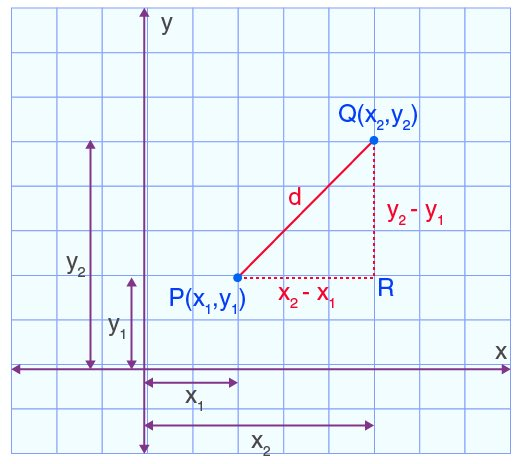
\includegraphics[width=0.7\linewidth]{EDistance.jpg}
    \caption{Euclidean Distance}
    \label{fig:enter-label}
\end{figure}


Euclidean distance is the shortest distance between two points means the straight line between source and destination whereas the Manhattan distance is the sum of all the real distances between the source and destination. And each always be a straight line. The reason behind Euclidean distance used in KNN is that it provides a simple and intuitive measure of similarity between data points in a multi-dimensional space. One of the main reason is that Euclidean distance in KNN, is its computational efficiency and simplicity. Euclidean distance metric works well for contious features and 



Euclidean Distance is largely used in machine learning learning algorithms such as K-Nearest(KNN) where it is used to measure the similarity between two data points.Spatial Analysis for measuring distance between geographical locations. As well as, in robotics for obstacle avoidance and path planning. It is also used in image process for comparing images based on pixel values. 




 It is easy to compute and widely understood, making it a popular choice for measuring distances between points in machine learning algorithms.

Additionally, the Euclidean distance metric works well for continuous features and is suitable for data represented in a high-dimensional space. It captures the straight-line distance between points in space, which aligns with the intuitive notion of distance.

Furthermore, the Euclidean distance metric is invariant to the scale and orientation of the coordinate system, making it robust to transformations of the data.

Overall, the Euclidean distance metric is a versatile and effective choice for measuring distances between data points in KNN, making it a widely adopted approach in machine learning applications.





\



\paragraph{\textbf{Manhattan distance (p=1)}}
In Manhattan distance, the absolute value is measured between two points. Manhattan is widely used as for resloving the problems related to geometry. We can say it as a ordinary distance between two points. Manhattan distance is also one of the popular and dominant distance metrics. The most common example is Uber app visualization with a grid and navigation via streets from one address to another illustration. Manhattan is widely used in cluster analysis. K-Means clustering algorithm is the common example where Manhattan distance is used. The second name of Manhattan Distance is city Block Distance. The simplest way to calculate the distance is to go horizontally and then vertically until you get from one point to the other between two points and go vertically instead of going in a straight line. 

The Manhattan Distance or City Block Distance determines the absolute difference among the pair of the coordinates. It might be surprising, but the simplest way of calculating the distance between two points is to go horizontally and then vertically until you get from one point to the other, instead of just going in a straight line. It is a simpler technique since it only needs you to subtract instead of performing more complicated calculations.

\begin{math}
 Manhattan distance = d(x,y)=\sqrt{(\sum_{i=1}^{m} |X_{i} - Y_{i})|)}
 \newline
\end{math}
As shown, it is the root of squared difference between the coordinates of two objects. We only need to subtract two points instead of performing complex tasks. 







\begin{figure}
    \centering
    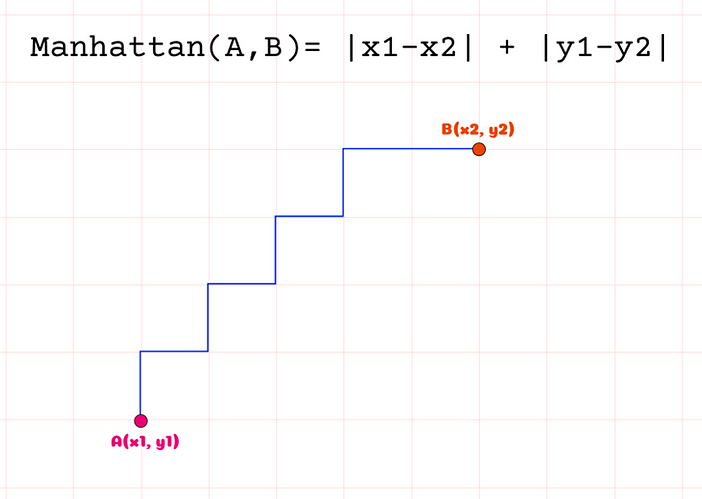
\includegraphics[width=0.8\linewidth]{a.png}
    \caption{Manhattan Distance}
    \label{fig:enter-label}
\end{figure}

\

\paragraph{\textbf{Minkowski distance}}
It is the generalized form of Manhattan and Euclidean distance matrics. Manhattan distance is denoted by p equal to one whereas the Euclidean distance is represented by p equal to two. Parameter p allows the creation of other distance metrics as shown below.

\begin{math}
 Minkowski distance =\sqrt{(\sum_{i=1}^{n} |X_{i} - Y_{i})|)^1/p}
 \newline
\end{math}

\begin{figure}
    \centering
    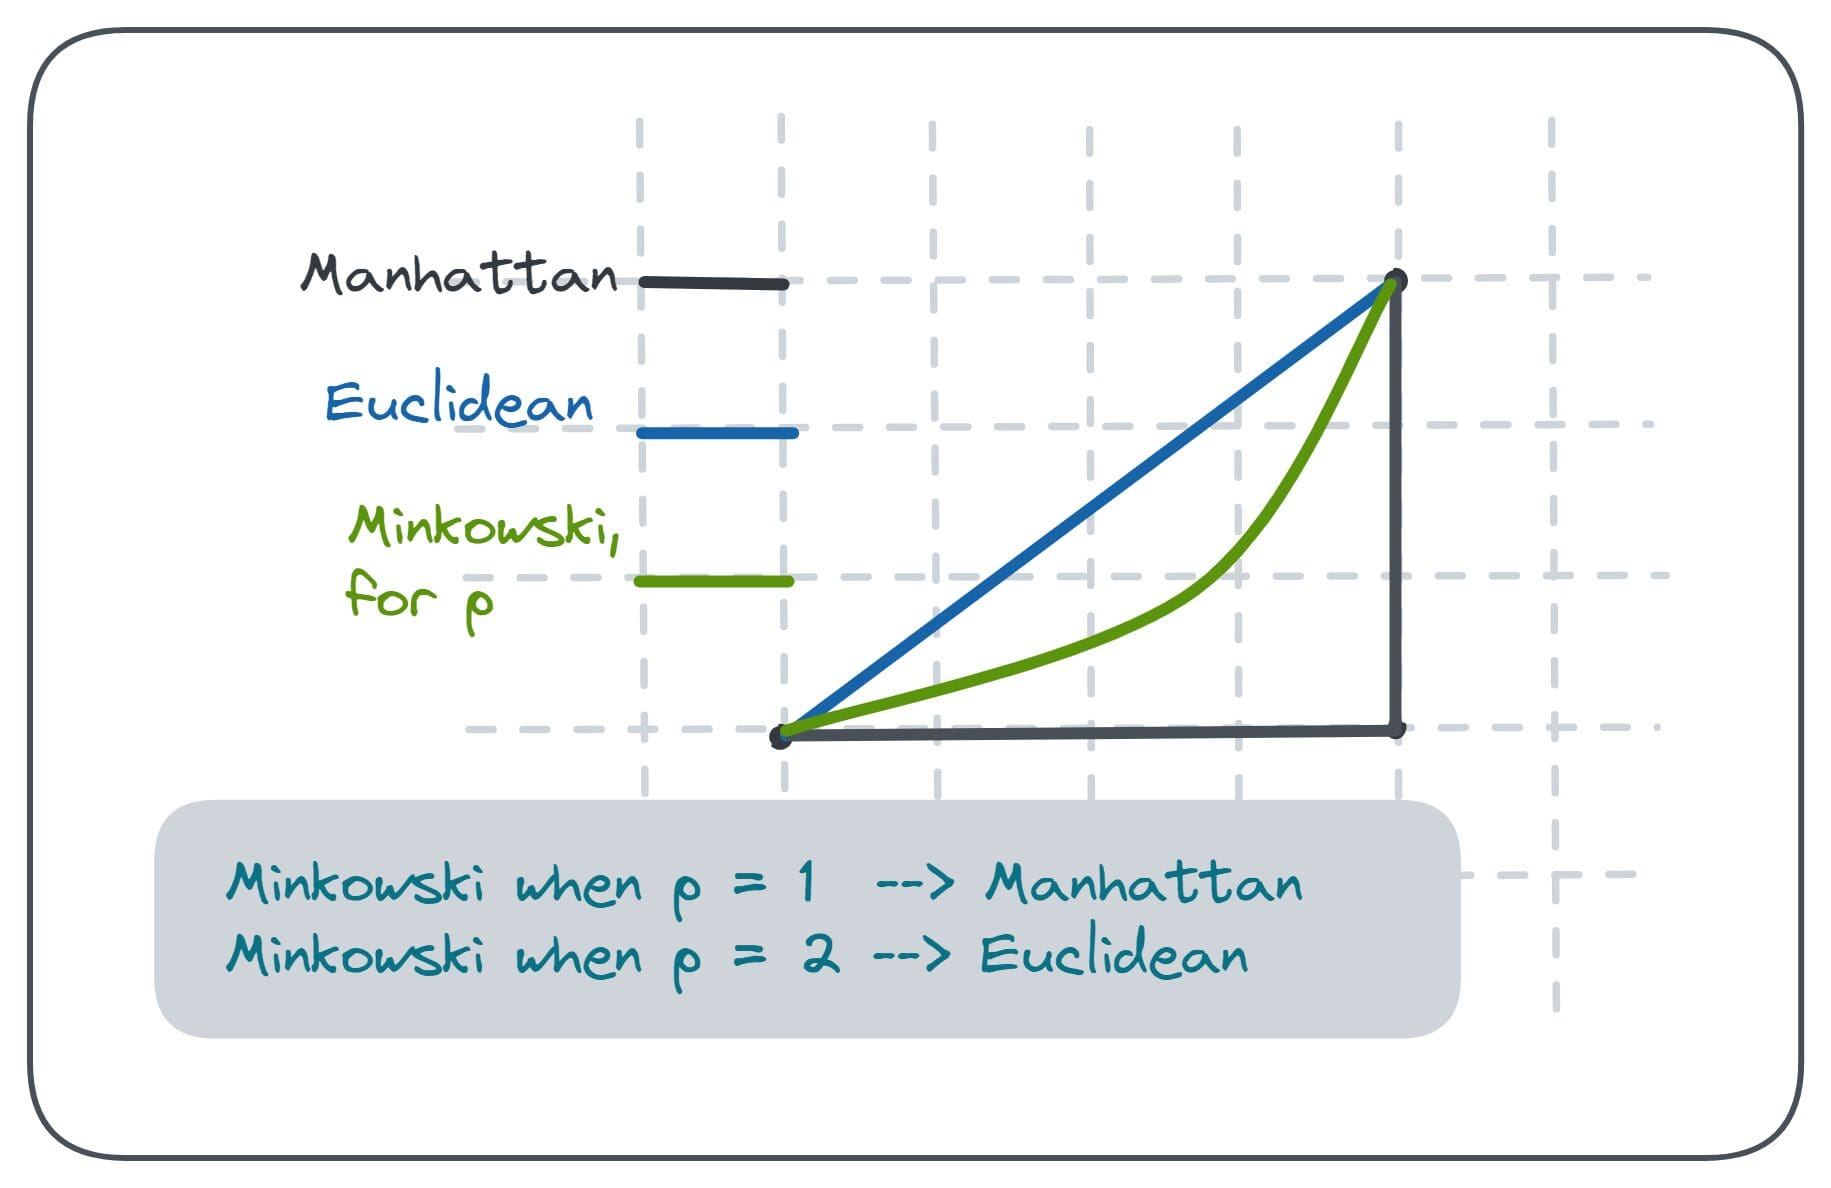
\includegraphics[width=0.8\linewidth]{b.jpg}
    \caption{Enter Caption}
    \label{fig:enter-label}
\end{figure}

\paragraph{\textbf{Hamming distance}}
This technique used with string vectors or boolean identifying the points where the vectors do not match. Overlap metrics are also referred as represented below:

\begin{math}
 Hamming Distance = D_{H}=(\sum_{i=1}^{k} |X_{i} - Y_{i})|)
 \newline
\end{math}



\subsubsection{Defining k selection}
In simple words, k is the number of neighors used for making predicition. The k value indicates how many neighbors will be compared or we can say checked to determine the resultant class in KNN Algorithm. For-example: By changing the value of k the classification can lead to underfitting or overfitting. If k=1, the instance will be assigned to the same class because we have a single neighbor. By using lower value of k can low bias, but high variance. As well as, larger value of k may lead to lower variance and high bias. So, we can define k as the balancing act as different values impact the variance on underfitting or overfitting. For avoiding ties in classification, k is recommended to be a odd number. The best approach to get a optimal k for you dataset is cross-validation tactics.  


\subsubsection{Voting Priniciple}




\begin{figure}
    \centering
    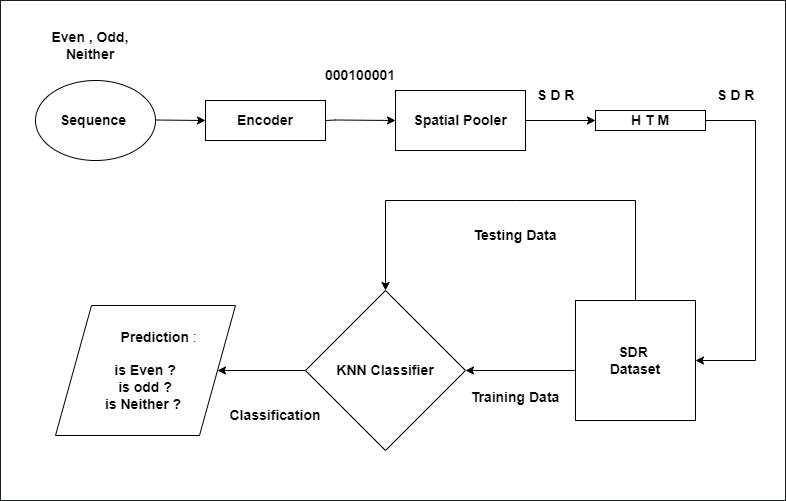
\includegraphics[width=1.0\linewidth]{Process Diagram.png}
    \caption{Process Diagram}
    \label{fig:enter-label}
\end{figure}



\subsection{Overview of HTM}
As the objective behind the HTM CLA is to make a progress towards making a program that functions cognitive tasks as like a simple human being brain. The prediction is done by making a system which can memorize as well as learn from the information executions which are fed before. HTM to anticipate and memorize, it requires user Input. 

As the overall HTM have multiple sections which includes data, Encoder, HTM spatial Pooler, HTM temporal Memory, and HTM Classifier. The data or which is also know as input is a scalar value, data or time, or a picture. Then the next element is encoder which is responsible for changing the data into SDR which can further be used with HTM classifier. SDR is in the cluster of binary input either '0' or '1'. As discussed earlier, input of encoder can be anything a scalar value. It includes locations, weeks, months, time or days in a week etc. 

The next part of the HTM is a spatial pooler it, is an algorithm which learns spatial patterns. The spatial pooler gets an input of bits cluster and converts it into SDR. Next Parts is Temporal memory, it a part which learns the arrangements of SDRs shaped by the spatial pooler algorithm. [5]  


\subsection{Spatial Pooler}
Spatial Poolar is the second phase of HTM learning. It uses the output of the encoder to learn the SDR of the given input binary array. The idea for the spatial poolar SDR is to generate SDRs of the input which is the output of the encoder. Once the input SDR are learned, if the same input is given again, it tries to match already learned SDRs and then generates a similar matching SDR.In this method, it will disgunish, is it a same input which is already memorized or a different one.   


\begin{figure}[h]
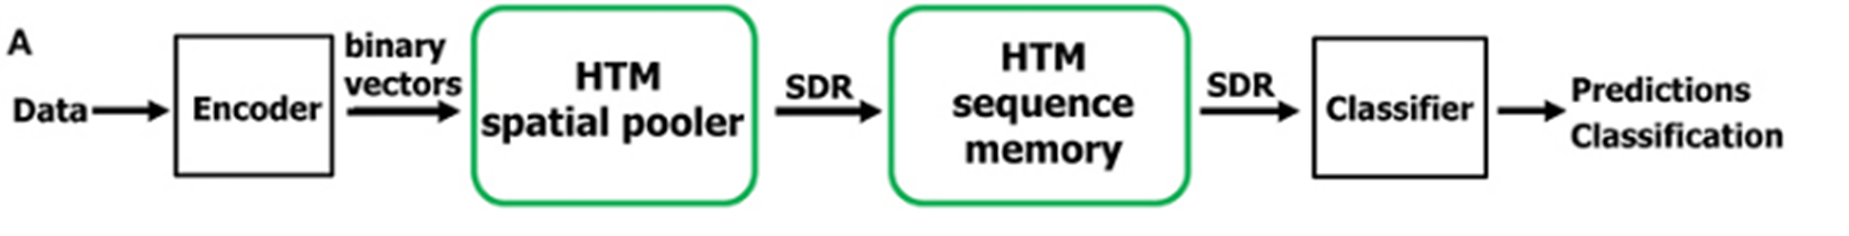
\includegraphics[scale=.40]{HtmPipeline.png}
\caption{General Flow}
\label{fig:enter-label}
\end{figure}






\section{Implementation Details}
The KNN method is divided into two classes first and main class is classifier which is consist of distnace, vote and classify. Second class for indexanddistance. Distance method which is used to calculate the distance of a new data point that has unlabeled data. The voting method is used to prepare the voting table from the distance matrix and the Classify method is used to classify the class of the unknown label data as an output. Remember we are using text file as our dataset which is slit into two parts training and test dataset. As these details are discussed in the further section in details. 


\subsection{Training and Test Dataset}
In the start, we have started with intilizing a array for the data matrix. But later-on we have created a text file from where we read the training data and test dataset. We have divided the file in such a way that 70\% of data act as a training data and other 30\% data in text file act as a test dataset. The large data sets, the technique is not scale able, due to fact that k-NN classifier store all the training data into memory. The below is example of our text file data. 
\begin{lstlisting}
04, 9697, 9772, 9841, 9851, 9922,........, 0
06, 9732, 9753, 9854, 9955, 10107,......., 0
10295, 10353, 10461, 10598, 10612,......., 1
06, 9854, 9881, 9955, 10107, 10165,......, 1
10792, 10812, 10880, 11007, 11060,......., 2
10418, 10662, 10777, 10846, 11008,......., 2
\end{lstlisting}
The starting value till the last index of each item are the predictor values and the last index is our class label. As we have there classes: the first one class is even numbers, second class is odd numbers elements and third class is decimal class which is also known as neither odd or even. The even class is represented by 0, odd class is represented by 1 and decimal class dataset is represented by 2. The second way to store class label is to introduce a separate array in which the class label will be stored. In our code we have assumed the class labels are numeric and the number starts from 0. 
\begin{lstlisting}
static int[] ExtractLabels(double[][] testData)
{
// Extract actual labels from the dataset
// Assuming labels are stored in the last 
// Column of each row
int[] actualLabels = new int[testData.Length];
for (int i = 0; i < testData.Length; i++)
{
actualLabels[i] = (int)testData[i].Last();
}
return actualLabels;
}
\end{lstlisting}

The above code is used for extracting label from the dataset. As we have already discussed that the label of class is the last index. And for extraction of that specific last index, the above piece of code is used. The next point is test data. In test data, which is 30\% of our file, is used to determine the accuraccy of our implementation. The classify function accepts multiple parameters fro the item to predict, it includes the number of classes in the training data as we have 3 classes, the number of nearest neighbors to evaluate and the matrix of training data, so the classifier is the function which determine or classify our data. Further discussed in the KNN implementation section. 





\subsection{KNN Impelementation}
In the high level, If I summerize the pseudo-code, there are only three major steps which includes:
\begin{lstlisting}
1. Compute distances from unknown
2. Sort the distances (nearest, farthest)
3. Use a vote to determine the result
\end{lstlisting}

These sections try to discuss the methods defined within the KNN classifier Class, these methods are discussed below:

\subsubsection{Distance(double[] vector1, double[] vector2)}
As we have discussed in section 2(A) regarding the Euclidean distance. The distance function calculates the Euclidean distance between two vectors which in our case are vector1 and vector2. As, the formula of Euclidean distance is to go through each element of a vector and compute the squared difference and then find the accumulative sum. And then finally finding the square root of the whole sum, represents the Euclidean distance between two vectors. 

\begin{lstlisting}
double sum = 0.0;
for (int i = 0; i < testData.Length; ++i)
{
double difference = testData[i]-trainData[i];
sum += difference*difference;
}
return Math.Sqrt(sum);
\end{lstlisting}

This is a simple implementation of distance finding by Euclidean. We can also use other alternatives including Mahalanobis distance, Mahattan distance. K-NN is not good for mixed numerical and non-numerical data(categorical data), as K-NN needs a two notion "nearest" and most distance metrics to work so it strictly works on either numerical data or non-numeric data.  





\subsubsection{Vote(IndexAndDistance[] info, double[][] trainData, int numClasses, int k)}
This method performs the voting mechanism between the k nearest neighbors. The arguments of this method are IndexAndDistance which represents distance and Indices of nearest neighbors in other we can say the information of nearest neighbors, then our training dataset (trainData), the total number of classes (numClasses), and the value of K. The step of Vote method is to initialize an array whose responsibility is to store the total number of votes against each class means every nearest k-neighbour has a vote. In the starting the array is initialized as zero. Then in the second step, it goes through the first k neighbors and retrieves its class label from the training data, and the respective array index is counted as one positive vote. In our case, the training data have either an odd number or an even number respective voting has been counted for each of them. Then the counted voting with the highest vote returns its label as the predicted class. 

\begin{lstlisting}
static int Vote(IndexAndDistance[] info, double[][] trainData, int numofclass, int k)
    {
        int[] votes = new int[numofclass];

        for (int i = 0; i < numofclass; ++i)
         {
          votes[i] = 0;
         }

        for (int i = 0; i < k; ++i)
         {
          int idx = info[i].idx;
          int c = (int)trainData[idx][20];
          ++votes[c];
          }
        int mostVotes = 0;
        int classWithMostVotes = 0;

            // Loop through each class
        for (int j = 0; j < numofclass; ++j)
        {
            if (votes[j] > mostVotes)
            {
                 
              mostVotes = votes[j];
              classWithMostVotes = j;
            }
        }

            return classWithMostVotes;
    }



\end{lstlisting}


As, we know that finding a class label is little bit trickier from the k items. As above code shows every k-nearest training gets one vote for its class label. In the start votes is intilized as zero. Then it add if class is nearest.  As currently we also have to count the votes. So, the class which have higher number of vote is the class from where our test data belongs from that specific class. It can be either odd, even or decimal class. 





\subsubsection{Classifier(double[] unknownSDR, double[][] Sdrdata, int numofclass, int k)}
This method performs the KNN classification for a given unknown SDR which we are also saying as test-data. The arguments of this method include the testdata (unknownSDR) and the training data (Sdrdata) and the total number of classes which is 3 in our case. And the value of k as an input parameter. In this method, we have called all the methods including IndexandDistance objects to store indices and distances of all data points from the unknown SDR. The next, we have called the distance method, which will calculate the distances between the test data ad training data points that are stored in the array. Then we sorted an array in ascending order based on distances. Then in the final, we have called the vote method to determine the predicted class label based on k nearest neighbors. Then, the class with the highest vote is where the test data belongs to that specific class. And then this method returns the result of a specific class label. 


\subsubsection{IndexAndDistance Class}
This class used to represent the index of a training item and its distance from the input (test data). It implements the IComparable<IndexAndDistance> Interface to enable sorting based on distance. The CompareTo method is overridden to compare distances between instances of the IndexAndDistance class.


\begin{figure}
    \centering
    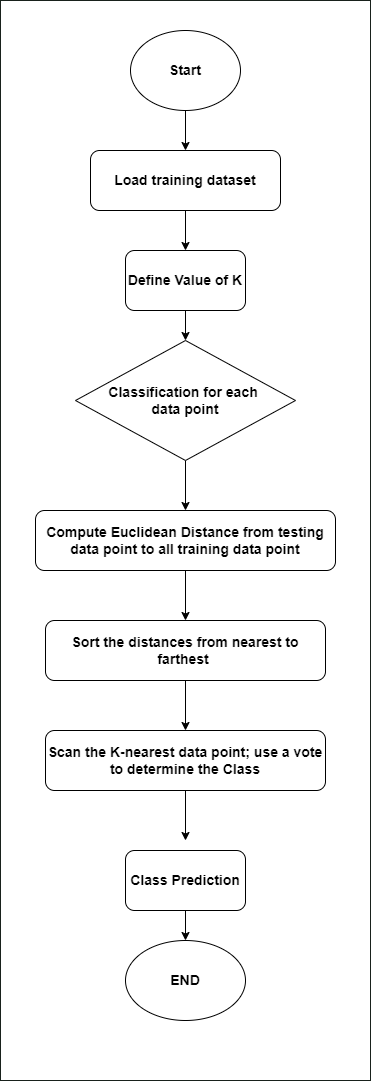
\includegraphics[width=0.5\linewidth]{KNNClassifier.png}
    \caption{KNN Flow Diagram according to steps}
    \label{fig:enter-label}
\end{figure}




\subsection{Unit Testing and Exception Handling}
Overview of unit testing methodologies used.
Description of UnitTest1 class and its purpose.
Explanation of how test datasets are generated and utilized for testing.
Discussion of exception handling strategies implemented.
Explanation of how errors and exceptions are handled during file reading and data parsing.


%Explanation of how SDR datasets are handled and utilized.
%Description of methods for loading SDR data from files.
%Discussion of data structures and formats used for SDR datasets.


\section{Results}
ALL the results should be here. 

\section{Discussion}

\subsection{Design Challenges}


\subsection{Applications of k-NN in machine learning}
KNN Algorithm is utilized in different applications across different sectors, mostly in classification. The common cases includes:


\subsubsection{Pattern Recognition}
KNN is used for the identification of specific patterns, it can be in a text. Like it predict the missing fill-in-the-blanks. This also help in solving cache which are basically handwritten numbers. So, KNN can also
to identify these patterns.


\subsubsection{Healthcare}
The common use of KNN is health department is prediction of chances of cancer as well as heart attacks risks. The algorithm try to learn from most likely gene expressions. 

\subsubsection{Recommendation Engines}
When we surf on internet, the KNN algorithm can be used by the website to recommend us other additional content. This recommendation is based on user behaviour. But for larger datasets this approach is not optimal. 

\subsubsection{Data preprocessing}
Mostly we have a missing values in our dataset, KNN algorithm can help to determine those values. Those estimated missing values are also known as missing data imputation. 

\subsubsection{Finance}
The banks uses the credit card spending to predict the risk associated with the specific individual loan. As well as knn is used to determine the credit card worthiness of a loan application. So, KNN is used in a variety of economic and finance departments. As well as the other common use case is currency exchange forecasting, stock market as well as trading futures etc.  



\section{Conclusion}


% conference papers do not normally have an appendix


% use section* for acknowledgment
\section*{Acknowledgment}


The authors would like to thank...





% trigger a \newpage just before the given reference
% number - used to balance the columns on the last page
% adjust value as needed - may need to be readjusted if
% the document is modified later
%\IEEEtriggeratref{8}
% The "triggered" command can be changed if desired:
%\IEEEtriggercmd{\enlargethispage{-5in}}

% references section

% can use a bibliography generated by BibTeX as a .bbl file
% BibTeX documentation can be easily obtained at:
% http://mirror.ctan.org/biblio/bibtex/contrib/doc/
% The IEEEtran BibTeX style support page is at:
% http://www.michaelshell.org/tex/ieeetran/bibtex/
%\bibliographystyle{IEEEtran}
% argument is your BibTeX string definitions and bibliography database(s)
%\bibliography{IEEEabrv,../bib/paper}
%
% <OR> manually copy in the resultant .bbl file
% set second argument of \begin to the number of references
% (used to reserve space for the reference number labels box)
\begin{thebibliography}{1}

\bibitem{1}
Cover, T., \& Hart, P. (1967). Nearest neighbor pattern classification. IEEE transactions on information theory, 13(1), 21-27.

\bibitem{2}
J. Z. A. L. J. W. Q. and L. S. Zhang, "An adaptive KNN algorithm based on data point density," IEEE Access, 7, 80876-80883. doi: 10.1109/ACCESS.2019.2926611, 2019.


\bibitem{4}
S. A. a. J. H. Y. Cui, "Continuous Online Sequence Learning with an Unsupervised Neural Network Model," Neural Comut.,, vol. 28, pp. 2474-2504, 2016.





%corrected

\bibitem{8}
X. L. Y. and C. Z. Yu, "Weighted K-nearest neighbor algorithm based on Gaussian kernel function," Journal of Ambient Intelligence and Humanized Computing, 11(5), 1985-1993. doi: 10.1007/s12652-019-01633-9, 2020.

\bibitem{9}
Taunk, Kashvi and De, Sanjukta and Verma, Srishti and Swetapadma, Aleena. (2019). A Brief Review of Nearest Neighbor Algorithm for Learning and Classification. 1255-1260. 10.1109/ICCS45141.2019.9065747. 


\bibitem{10}
Song Yang, Jian Huang, Ding Zhou, Hongyuan Zha, and C. Lee Giles, “Iknn:
Informative k-nearest neighbour pattern classification,” in Knowledge Discovery in Databases, (2007), pg. 248– 264.


\bibitem{11}
Han EH.., Karypis G., Kumar V.(2001) “Text Categorization Using Weight Adjusted k-Nearest Neighbour Classification”. In: Cheung D., Williams G.J., Li Q. (eds) Advances in Knowledge Discovery and Data Mining. PAKDD 2001. Lecture Notes in Computer Science, vol 2035. Springer, Berlin, Heidelberg.



\bibitem{12}
D. Wettschereck and D. Thomas G., “Locally adaptive nearest neighbour algorithms,” Adv. Neural Inf. Process. Syst., pg. 184–186, 1994.





\end{thebibliography}




% that's all folks
\end{document}


